\section{Ultrasonic Sensor HC-SR04}
\begin{figure}[ht]
\centerline{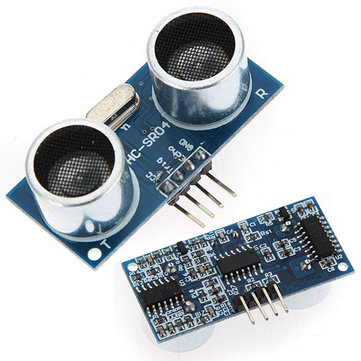
\includegraphics[width=0.5\textwidth]{figures/sensor.jpg}}
\caption{Sensor Ultrasonic SR04}
\label{sensor}
\end{figure}
\subsection{Penjelasan}
Ultrasonic Sensor (Gambar \ref{sensor}) adalah sensor yang mengukur jarak dengan menggunakan sensor ultrasonic. Sensor tersebut mentransmisikan gelombang ultrasonik dan menerima pantulan dari gelombang ultrasonik dari benda di depannya. 
\subsection{Penggunaan Sensor Ultrasonic}
Sensor Ultrasonic (Gambar \ref{sensor}) telah dipakai di berbagai perangkat atau platform yang memiliki berbagai kegunaan, diantaranya sebagai berikut : 
\begin{itemize}
	\item Sebagai pengukur kedalaman air \\ Gelombang yang dihasilkan oleh sensor dapat merambat melalui air dan memantulkannya kembali sehingga dapat mengembalikan hasil yang akurat dari sensor.
	\item Sebagai membantu proses parkir mobil \\  Dengan dipasang sensor tersebut dapat mengukur jarak antara mobil dengan tembok di belakang atau depan mobil tersebut.
	\item Sebagai sensor benda pada Robot \\ \cite{ruan2014ultrasonic} Dengan dipasang sensor ini dapat membuat sebuah robot mengetahui jika ada benda di depannya dan akan dapat dihindari benda tersebut.
\end{itemize}
\subsection{Contoh Project Sensor}
\subsubsection{Perakitan Sensor}
Berikut adalah contoh project Sensor yang telah dilakukan.\\\\ Barang yang dibutuhkan : 
\begin{itemize}
	\item Kabel Jumper x10 atau lebih
	\item Lampu LED x1
	\item Ultrasonic Sensor HC-SR04 x1
	\item Arduino UNO x1 atau Arduino jenis Lainnya (Disarankan Arduino UNO)
	\item Resistor 220ohm x1 atau lebih
	\item Piezo Buzzer/Buzzer x1
	\item Arduino IDE (Download in PC)
\end{itemize}
Langkah - langkah merakit : 
\begin{enumerate}
	\item Hubungkan Arduino dengan sensor dan barang lainnya. Hubungan kabel (Arduino to Barang) seperti gambar dibawah : 
\begin{figure}[ht]
\centerline{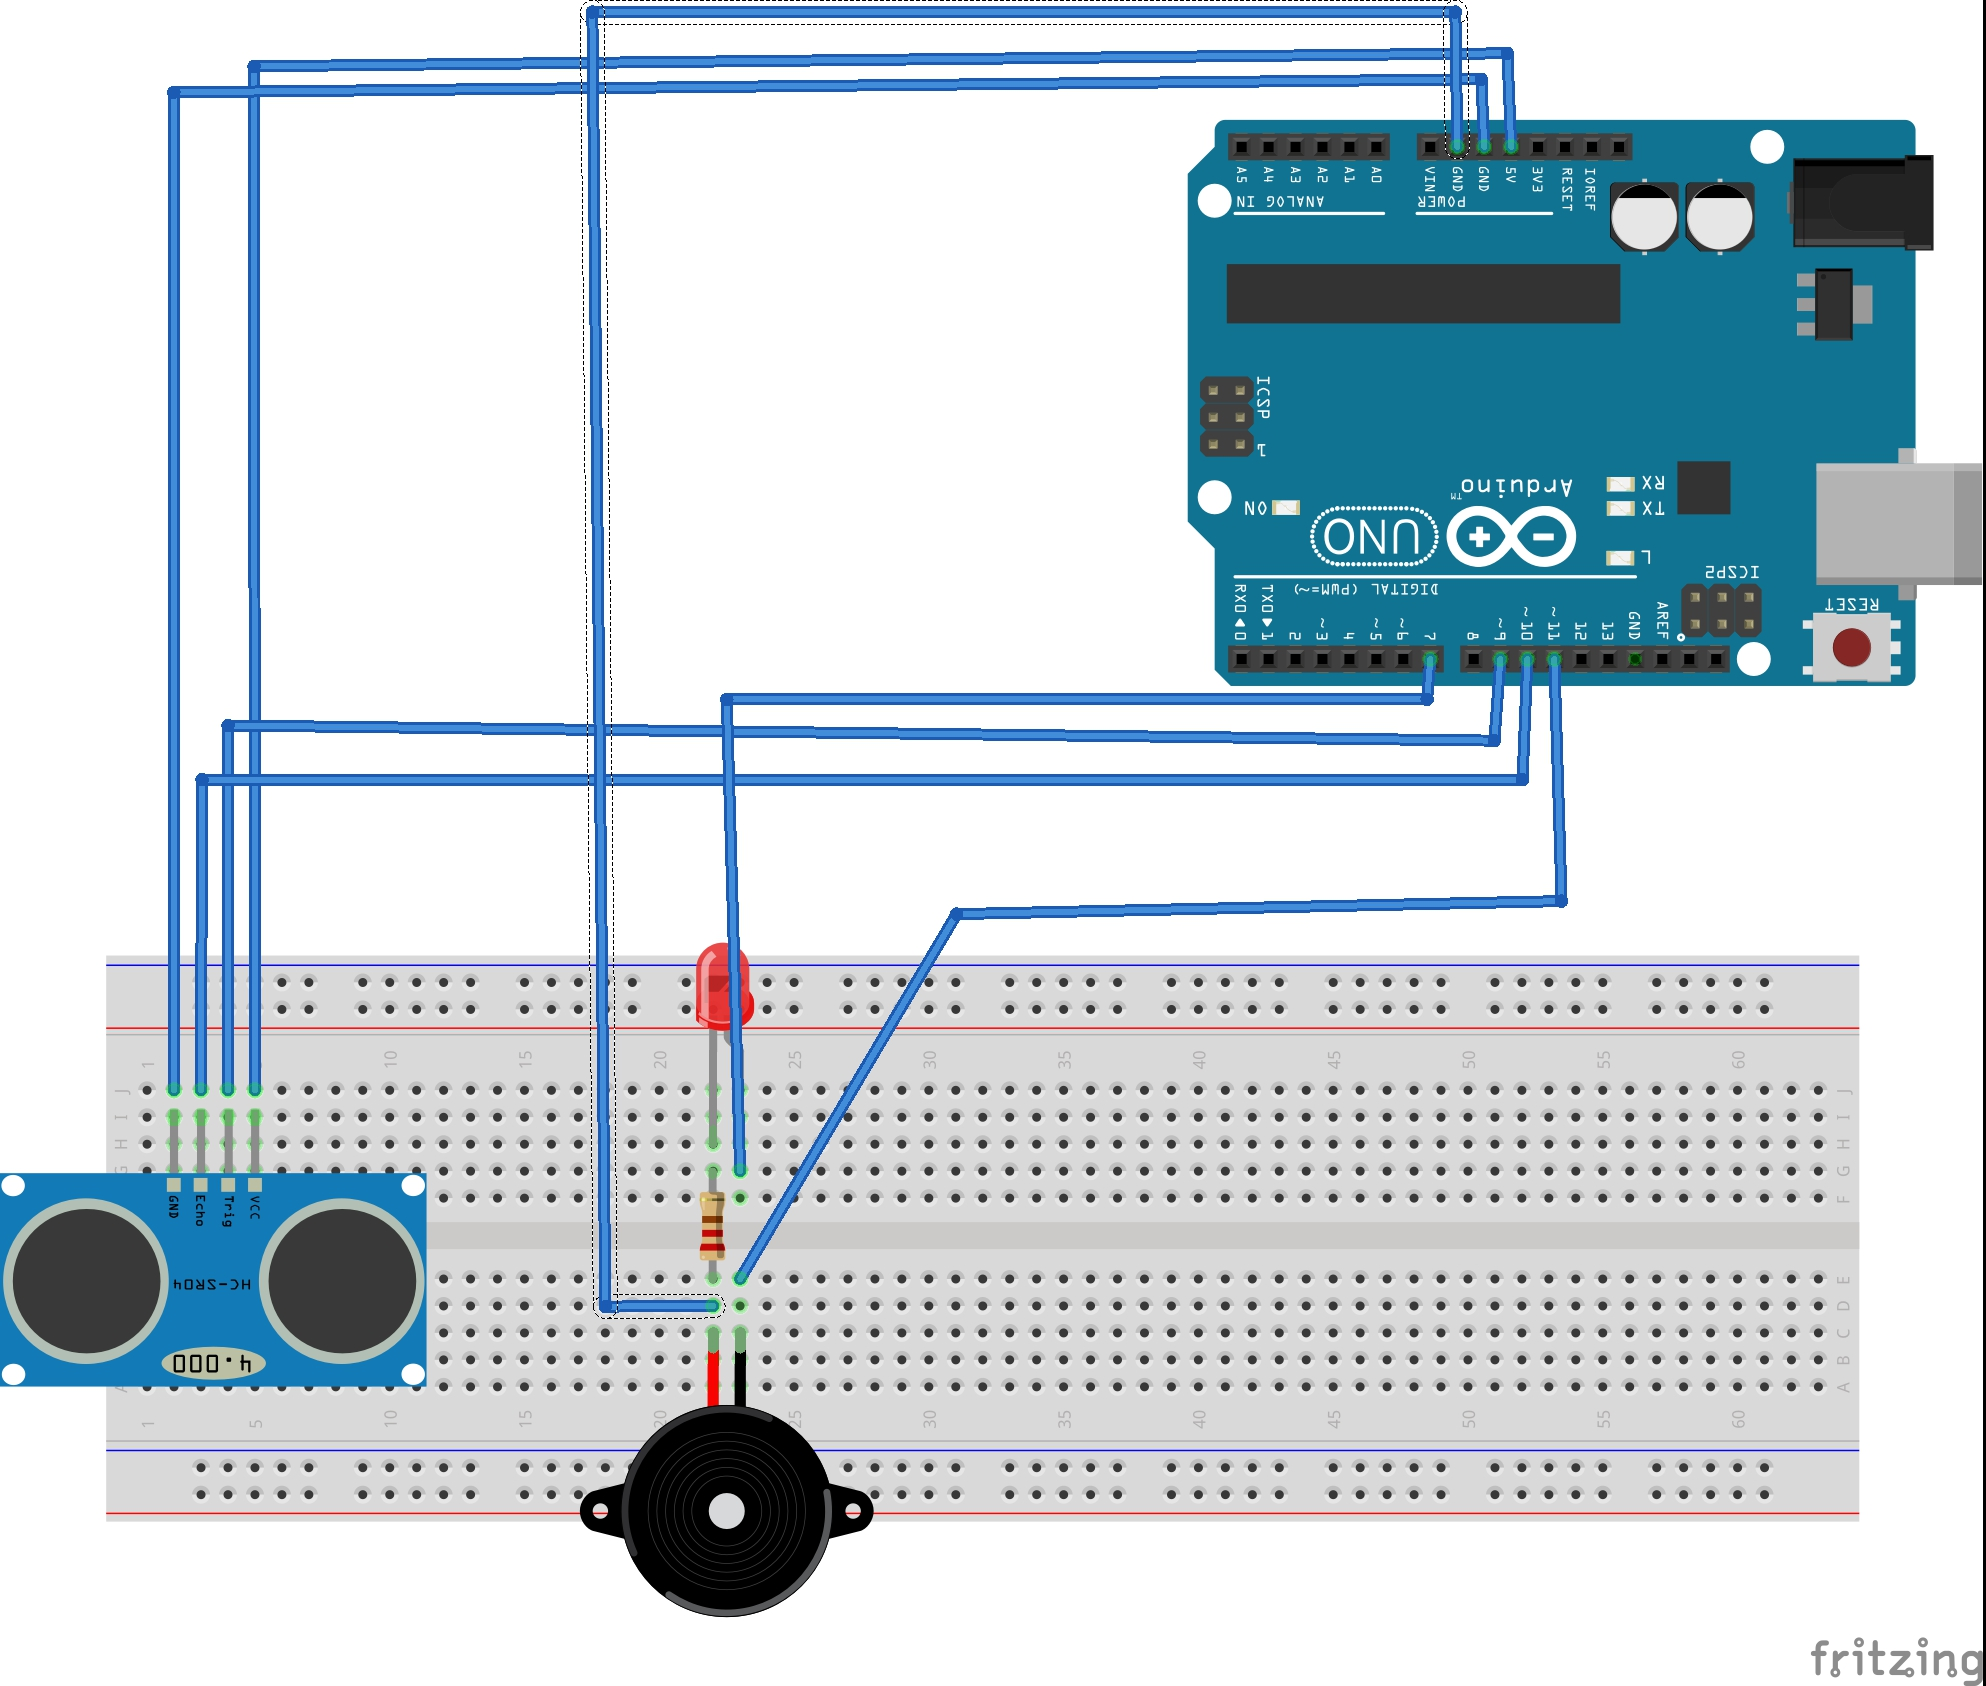
\includegraphics[width=1\textwidth]{figures/rancangan.jpg}}
\caption{Rancangan Kabel}
\label{rancangankabel}
\end{figure}
		\begin{itemize}
			\item GND to SR04 GND
			\item Pin 10 to SR04 Echo
			\item Pin 09 to SR04 Trig
			\item Pin 5V to SR04 VCC
			\item Pin 11 to Buzzer Anode(+)
			\item GND to Buzzer Cathode(-)
			\item Buzzer Cathode Resistor to LED Cathode
			\item Pin 07 to LED Anode
		\end{itemize}
	\item Masukan Kode berikut pada Arduino IDE : 
\begingroup\makeatletter\def\@currenvir{verbatim}
\verbatim
    /*
    * Ultrasonic Sensor HC-SR04 and Arduino Tutorial
    *
    * Crated by Dejan Nedelkovski,
    * www.HowToMechatronics.com
    *
    */
    // defines pins numbers
    const int trigPin = 9;
    const int echoPin = 10;
    // defines variables
    long duration;
    int distance;
    void setup() {
    pinMode(trigPin, OUTPUT); // Sets the trigPin as an Output
    pinMode(echoPin, INPUT); // Sets the echoPin as an Input
    Serial.begin(9600); // Starts the serial communication
    }
    void loop() {
    // Clears the trigPin
    digitalWrite(trigPin, LOW);
    delayMicroseconds(2);
    // Sets the trigPin on HIGH state for 10 micro seconds
    digitalWrite(trigPin, HIGH);
    delayMicroseconds(10);
    digitalWrite(trigPin, LOW);
    // Reads the echoPin, returns the sound wave travel time in microseconds
    duration = pulseIn(echoPin, HIGH);
    // Calculating the distance    
    distance= duration*0.034/2;
    if(distance<30){
      digitalWrite(7, HIGH);
      tone(11, 2000);     
    }else{
      digitalWrite(7, LOW);
      noTone(11);
    }
    // Prints the distance on the Serial Monitor
    Serial.print("Distance: ");
    Serial.println(distance);
    }
\end{verbatim}
	\item Lalu Hubungkan Kabel USB dari Arduino ke komputer lalu Verify dan Compile
\end{enumerate}
\subsubsection{Hasil yang didapat dari Sensor}
Hasil dari project tersebut adalah dimana jika terdapat sebuah benda berada kurang dari 30cm dari arah depan sensor, maka sensor tersebut akan membunyikan buzzer dan lampu LED. jika tidak maka buzzer akan dimatikan dan lampu led akan mati.
\begin{figure}[ht]
\centerline{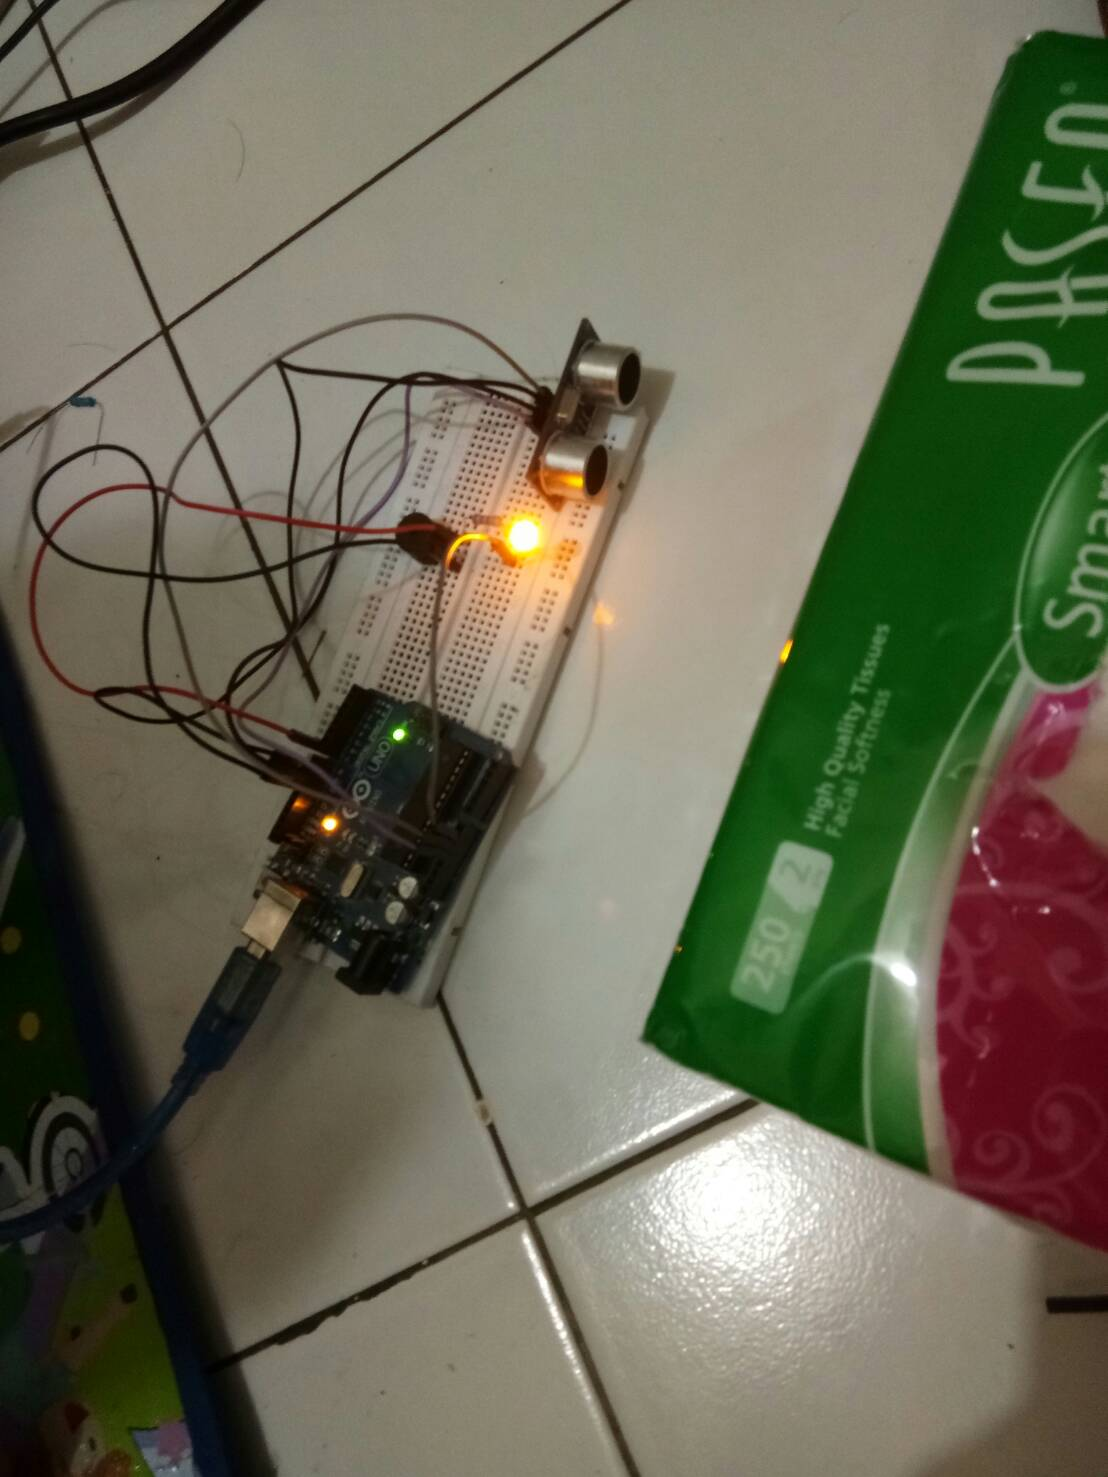
\includegraphics[width=0.6\textwidth]{figures/adabarang.jpg}}
\caption{Lampu menyala saat ada barang di depan dengan jarak 30cm}
\label{lampunyala}
\end{figure}
\begin{figure}[ht]
\centerline{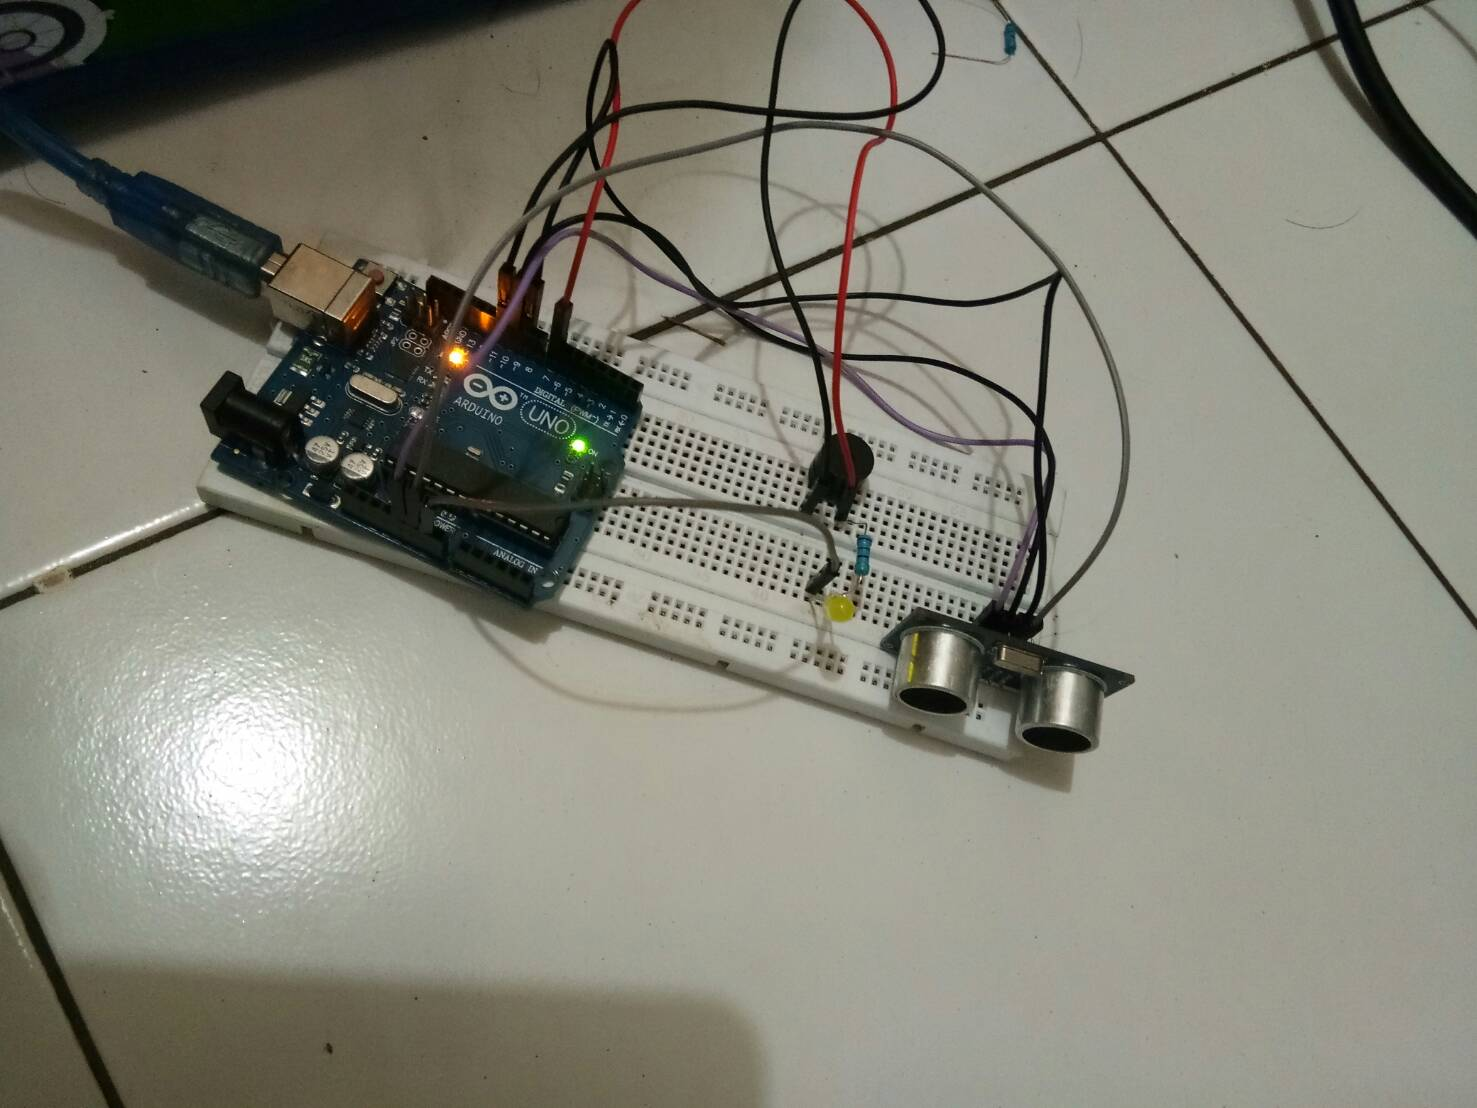
\includegraphics[width=1\textwidth]{figures/tidakada.jpg}}
\caption{Lampu mati saat tidak ada barang di depan dengan jarak 30cm}
\label{lampumati}
\end{figure}
\begin{figure}[ht]
\centerline{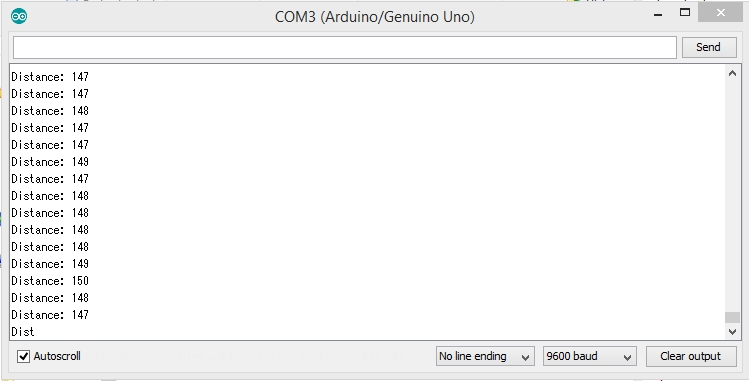
\includegraphics[width=1\textwidth]{figures/serialmonitorultrasonic.jpg}}
\caption{Hasil pada Serial Monitor}
\label{serialmonitor}
\end{figure}